\subsection{Challenges with secondary entry points}\label{subsection:applied-methods:prototypical-implementation:sharing
-secondary-entrypoints}

By default, all micro-frontend dependencies are shared through Module Federation. The required configuration options for every dependency in the micro-frontend architecture are \texttt{singleton}, \texttt{strictVersion}, and \texttt{requiredVersion}. These options are explained in more detail in Section \ref{subsection:background:micro-frontend:module-federation}. The versions of the dependencies are determined automatically from the \texttt{package.json}. However, some packages have problems being shared with these settings. The dependency \texttt{@apollo/client} is problematic because it has secondary entry points. When attempting to share \texttt{@apollo/client/core}, \texttt{@apollo/client/link/batch} and \texttt{@apollo/client/link/error} the warning message in Figure \ref{fig:applied-methods:sharing-secondary-entrypoints-error} is shown.

\ifshowImages
  \begin{figure}[H]
  \centering
  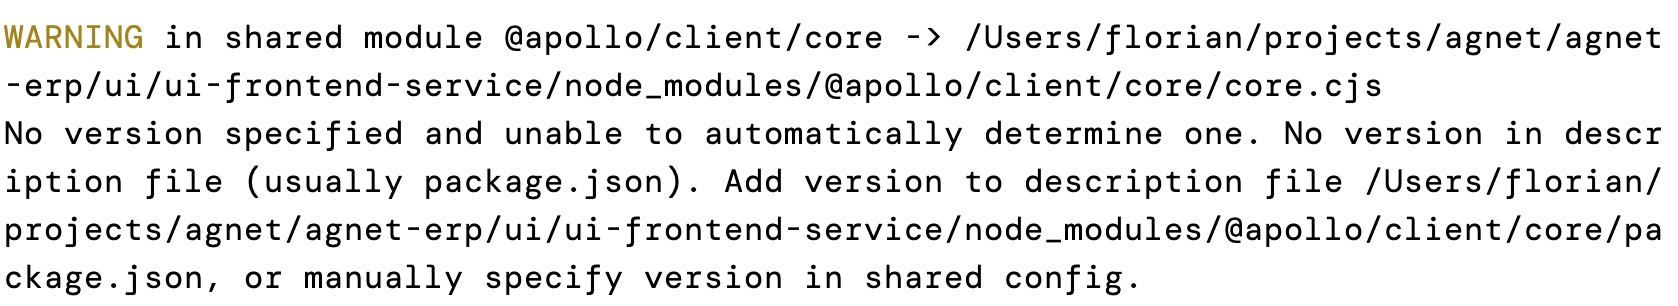
\includegraphics[width=1\linewidth]{images/applied-methods/prototypical-implementation/module-federation-apollo-warning.jpg}
  \caption{A warning message from Module Federation, that the \texttt{@apollo/client} dependency could not be shared.}\label{fig:applied-methods:sharing-secondary-entrypoints-error}
  \end{figure}
\fi

\noindent The root of the problems are the secondary entry points like \texttt{@apollo/client/core}, which are like an npm package inside another npm package. The content of the \texttt{package.json} from \texttt{@apollo/client/core} is shown in Listing \ref{code:applied-methods:package-json-apollo-client-core}. Webpack tries to resolve the version of the secondary entry point from that \texttt{package.json} and not from \texttt{@apollo/client}. The version is missing inside the file, so Webpack cannot determine the version and prints the warning message shown in Figure \ref{fig:applied-methods:sharing-secondary-entrypoints-error}. The warning does not lead to an error in production, but the dependencies cannot be shared and are included in every micro-frontend bundle.

\ifshowListings
\begin{listing}[H]
  \begin{minted}{json}
{
  "name": "@apollo/client/core",
  "type": "module",
  "main": "error.cjs",
  "module": "index.js",
  "types": "index.d.ts",
  "sideEffects": false
}
  \end{minted}
  \caption{The content of \texttt{package.json} from \texttt{@apollo/client/core}.}\label{code:applied-methods:package-json-apollo-client-core}
\end{listing}
\fi

\noindent The warning was fixed by specifying the version for these packages manually. The version is the same as that of \texttt{@apollo/client}. The configuration for sharing these packages is shown in the Listing \ref{code:applied-methods:sharing-secondary-entrypoints-config}. Everytime a package starts with \texttt{@apollo/client/} the version is set to \texttt{\^3.6.9}. This version is the same as the version of \texttt{@apollo/client}.

\ifshowListings
\begin{listing}[H]
  \begin{minted}{typescript}
shared: (libraryName, defaultConfig) => {
  if (libraryName.includes('@apollo/client/'))
    return { ...defaultConfig, version: '^3.6.9' };

  return defaultConfig;
}
  \end{minted}
  \caption{Specify the version for the secondary entry points for the \texttt{@apollo/client} package.}\label{code:applied-methods:sharing-secondary-entrypoints-config}
\end{listing}
\fi
